% Created 2019-09-29 Sun 13:38
% Intended LaTeX compiler: pdflatex
\documentclass[11pt]{article}
\usepackage[utf8]{inputenc}
\usepackage[T1]{fontenc}
\usepackage{graphicx}
\usepackage{grffile}
\usepackage{longtable}
\usepackage{wrapfig}
\usepackage{rotating}
\usepackage[normalem]{ulem}
\usepackage{amsmath}
\usepackage{textcomp}
\usepackage{amssymb}
\usepackage{capt-of}
\usepackage{hyperref}
\author{Dustin Leatherman}
\date{\today}
\title{Homework \#3}
\hypersetup{
 pdfauthor={Dustin Leatherman},
 pdftitle={Homework \#3},
 pdfkeywords={},
 pdfsubject={},
 pdfcreator={Emacs 26.3 (Org mode 9.2.4)}, 
 pdflang={English}}
\begin{document}

\maketitle
\tableofcontents


\section{2.23}
\label{sec:org2092d84}
\subsection{d}
\label{sec:orge48f418}
\begin{quote}
What is the absolute magnitude of the reduction in the variation of Y when X is
introduced into the regression model? What is the relative reduction? What is
the name of the latter measure?
\end{quote}

The absolute magnitude of the reduction in the variation of Y when X is
introduced is \(SSR = 3.588\).

The relative reduction in variance is \(R^2 = 0.0726\).
\subsection{e}
\label{sec:org6a14bd1}
\begin{quote}
Obtain r and attach appropriate sign
\end{quote}


\(r = \sqrt{R^2} = \sqrt{0.0726} = 0.2695\)
\subsection{f}
\label{sec:orgc1f08cf}
\emph{Which measure, \(R^2\) or \(r\) has the more clear-cut operational interpretation?}

\(R^2\) dictates the variance in Y explained by X and r measures the linear
association between Y and X. From an operational perspective, \(R^2\) is more
clear-cut as there is less interpretation required than the correlation
coefficient in which the sign is important.
\section{2.26}
\label{sec:org738deaa}
\subsection{c}
\label{sec:orge5d0a1e}
\begin{quote}
Plot the deviations \(Y_i - \hat{Y_i}\) against \(X_i\) on a graph. Plot the
deviations \(\hat{Y_i} - \bar{Y}\) on another graph. Does SSE or SSR appear to be
the larger component of SSTo? What does this imply about the magniture of
\(R^2\)?
\end{quote}

According to the two graphs, SSR appears to be a larger component of SSO. This
would mean that the magnitude of \(R^2\) is high.

\begin{figure}[htbp]
\centering
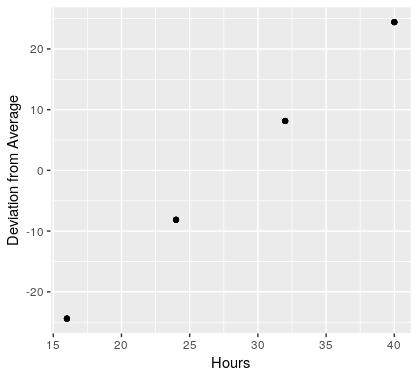
\includegraphics[width=.9\linewidth]{./images/2.26c_1.png}
\caption{\(Y_i - \bar{Y}\)}
\end{figure}

\begin{figure}[htbp]
\centering
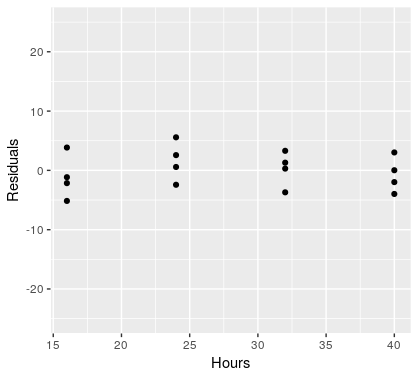
\includegraphics[width=.9\linewidth]{./images/2.26c_2.png}
\caption{Residuals}
\end{figure}
\subsection{d}
\label{sec:orgc6eec37}
\begin{quote}
Calculate \(R^2\) and \(r\)
\end{quote}


\begin{verbatim}
summary(plastic.model1)

#Call:
#lm(formula = Hardness ~ Hours, data = plastic)

#Residuals:
#    Min      1Q  Median      3Q     Max
#-5.1500 -2.2188  0.1625  2.6875  5.5750

#Coefficients:
#             Estimate Std. Error t value Pr(>|t|)
#(Intercept) 168.60000    2.65702   63.45  < 2e-16 ***
#Hours         2.03438    0.09039   22.51 2.16e-12 ***
#---
#Signif. codes:  0 ‘***’ 0.001 ‘**’ 0.01 ‘*’ 0.05 ‘.’ 0.1 ‘ ’ 1

#Residual standard error: 3.234 on 14 degrees of freedom
#Multiple R-squared:  0.9731,	Adjusted R-squared:  0.9712
#F-statistic: 506.5 on 1 and 14 DF,  p-value: 2.159e-12
\end{verbatim}



\(R^2 = 0.9731\)

\(r = \sqrt{R^2} = 0.9865\)
\section{3.2}
\label{sec:orgb4f023f}
\begin{quote}
Prepare a prototype residual plot for each of the following cases:
\begin{enumerate}
\item error variance decreases with X
\item true regression function is \(\cup\) shaped but a linear regression function
is fitted
\end{enumerate}
\end{quote}

\begin{figure}[htbp]
\centering
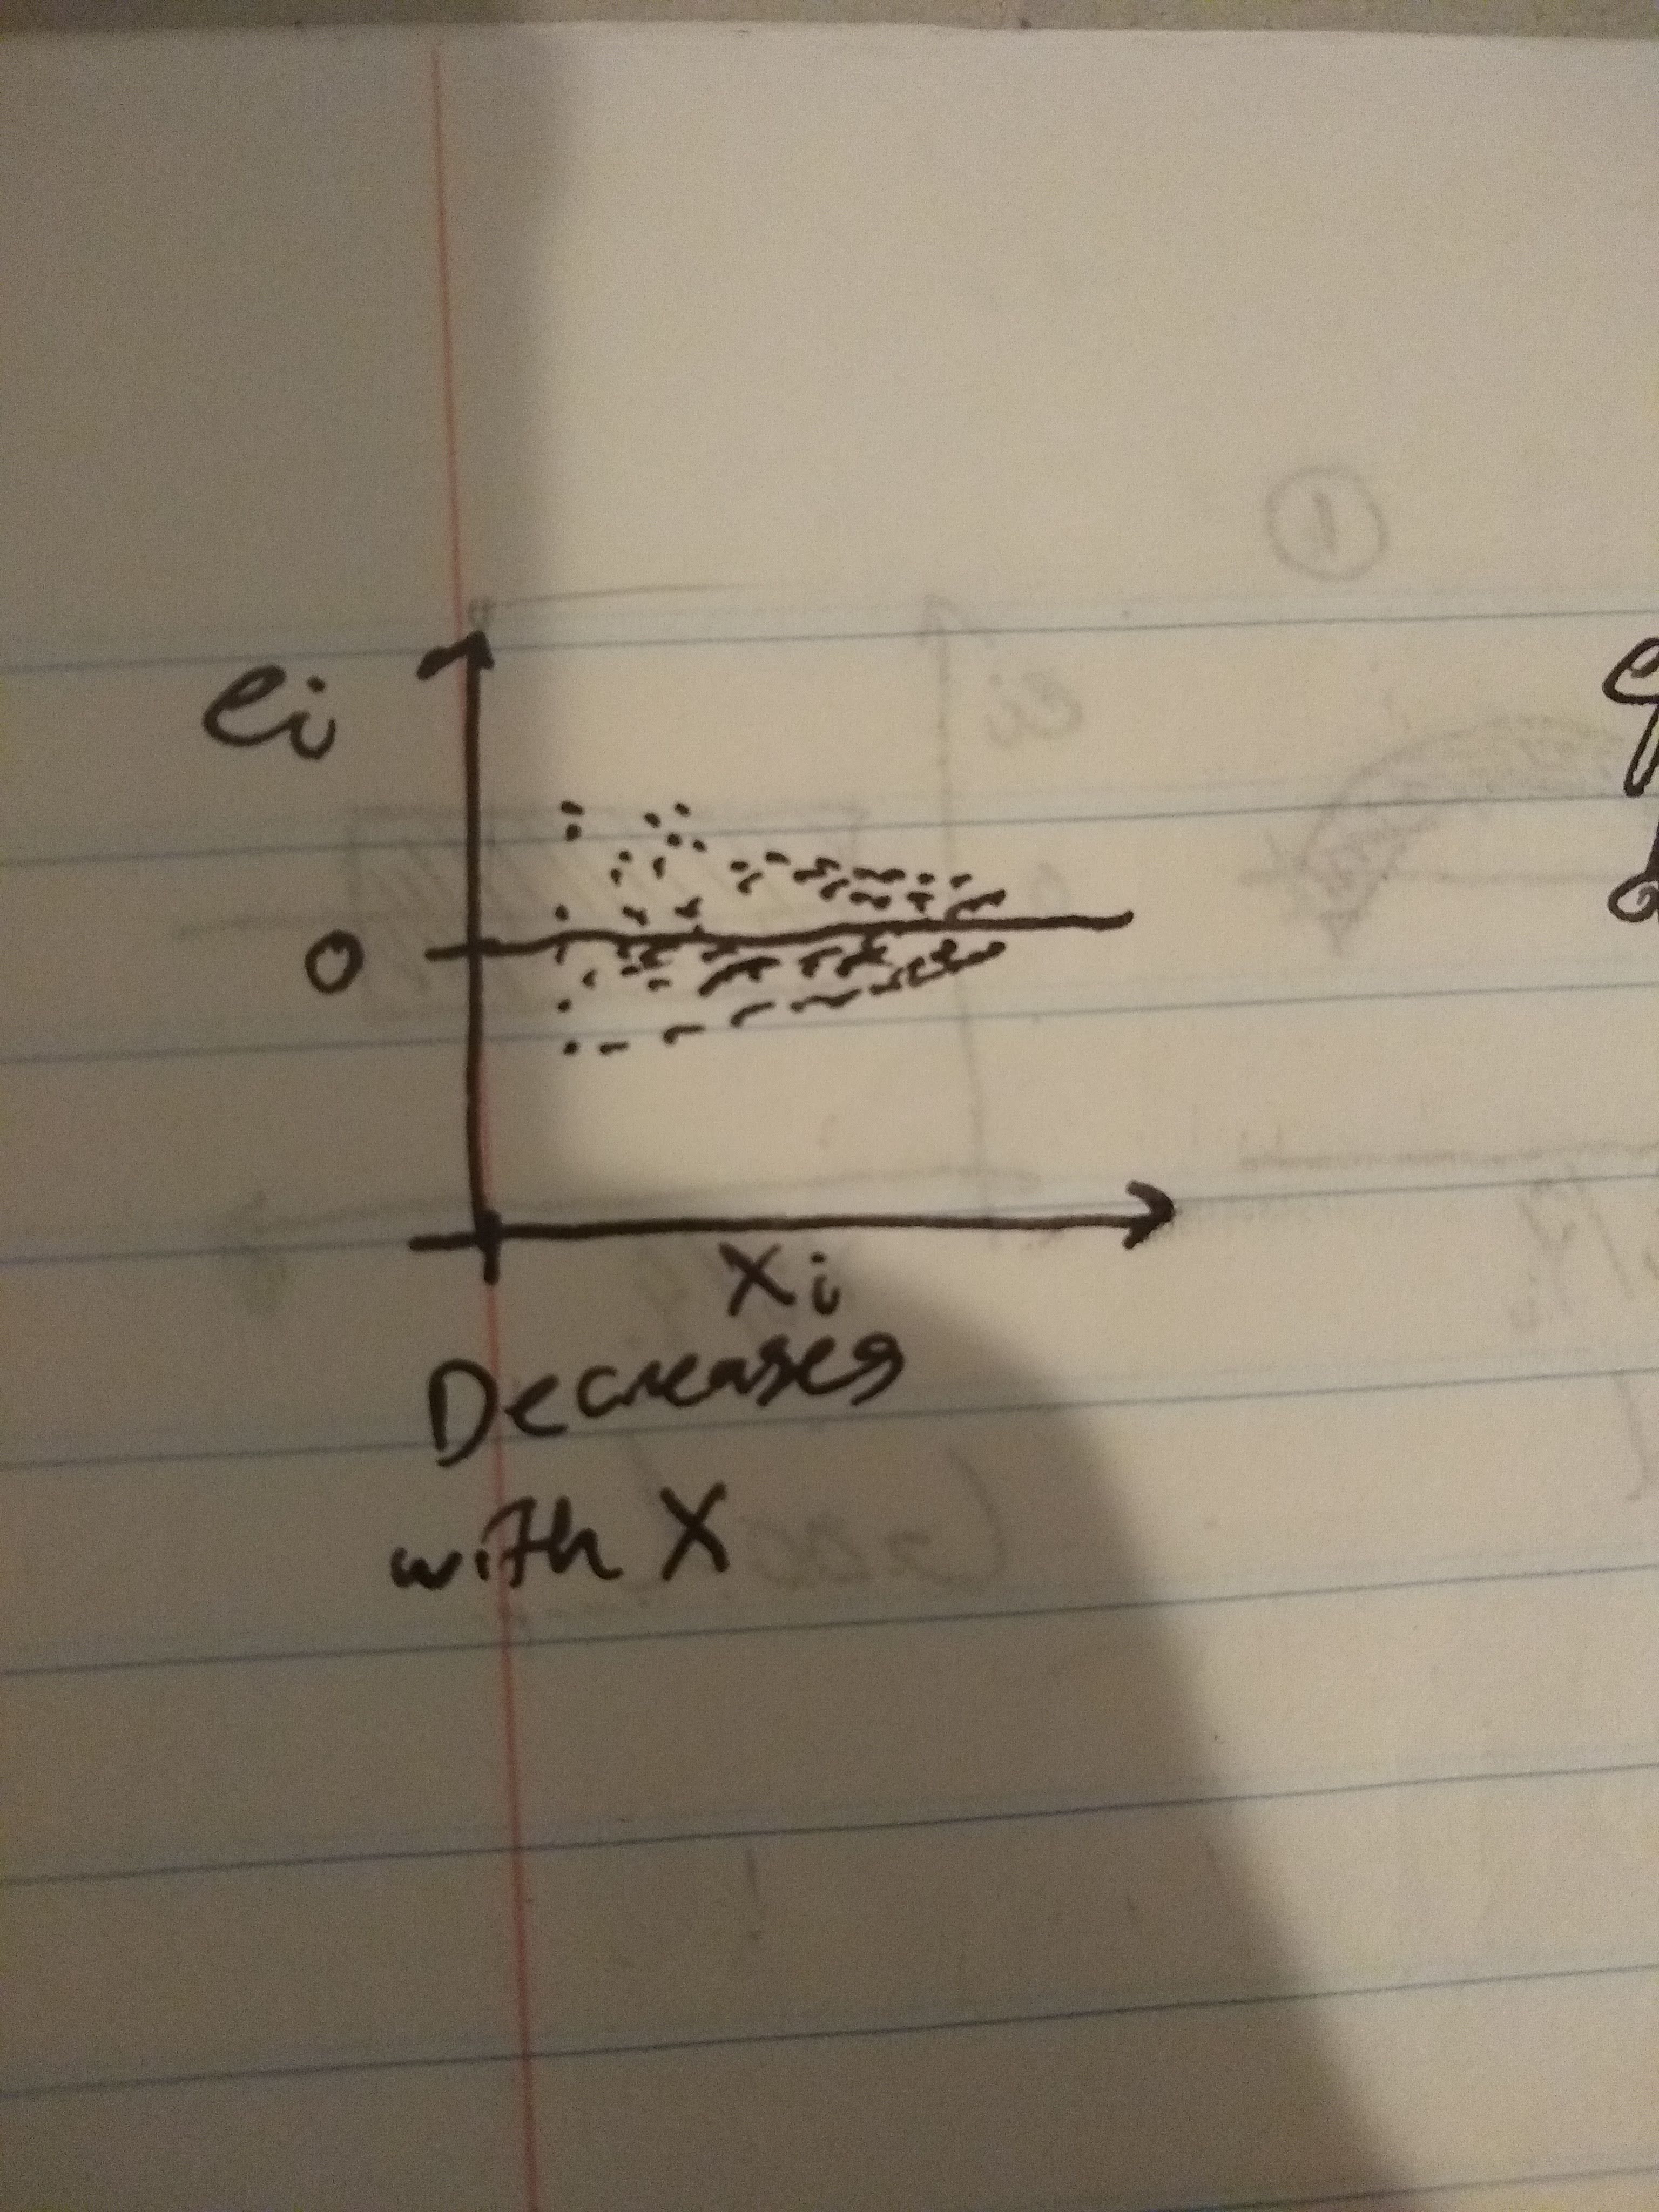
\includegraphics[width=.9\linewidth]{./images/3.2_1.jpg}
\caption{\label{fig:org28b4488}
Error Variance decreases with X}
\end{figure}

\begin{figure}[htbp]
\centering
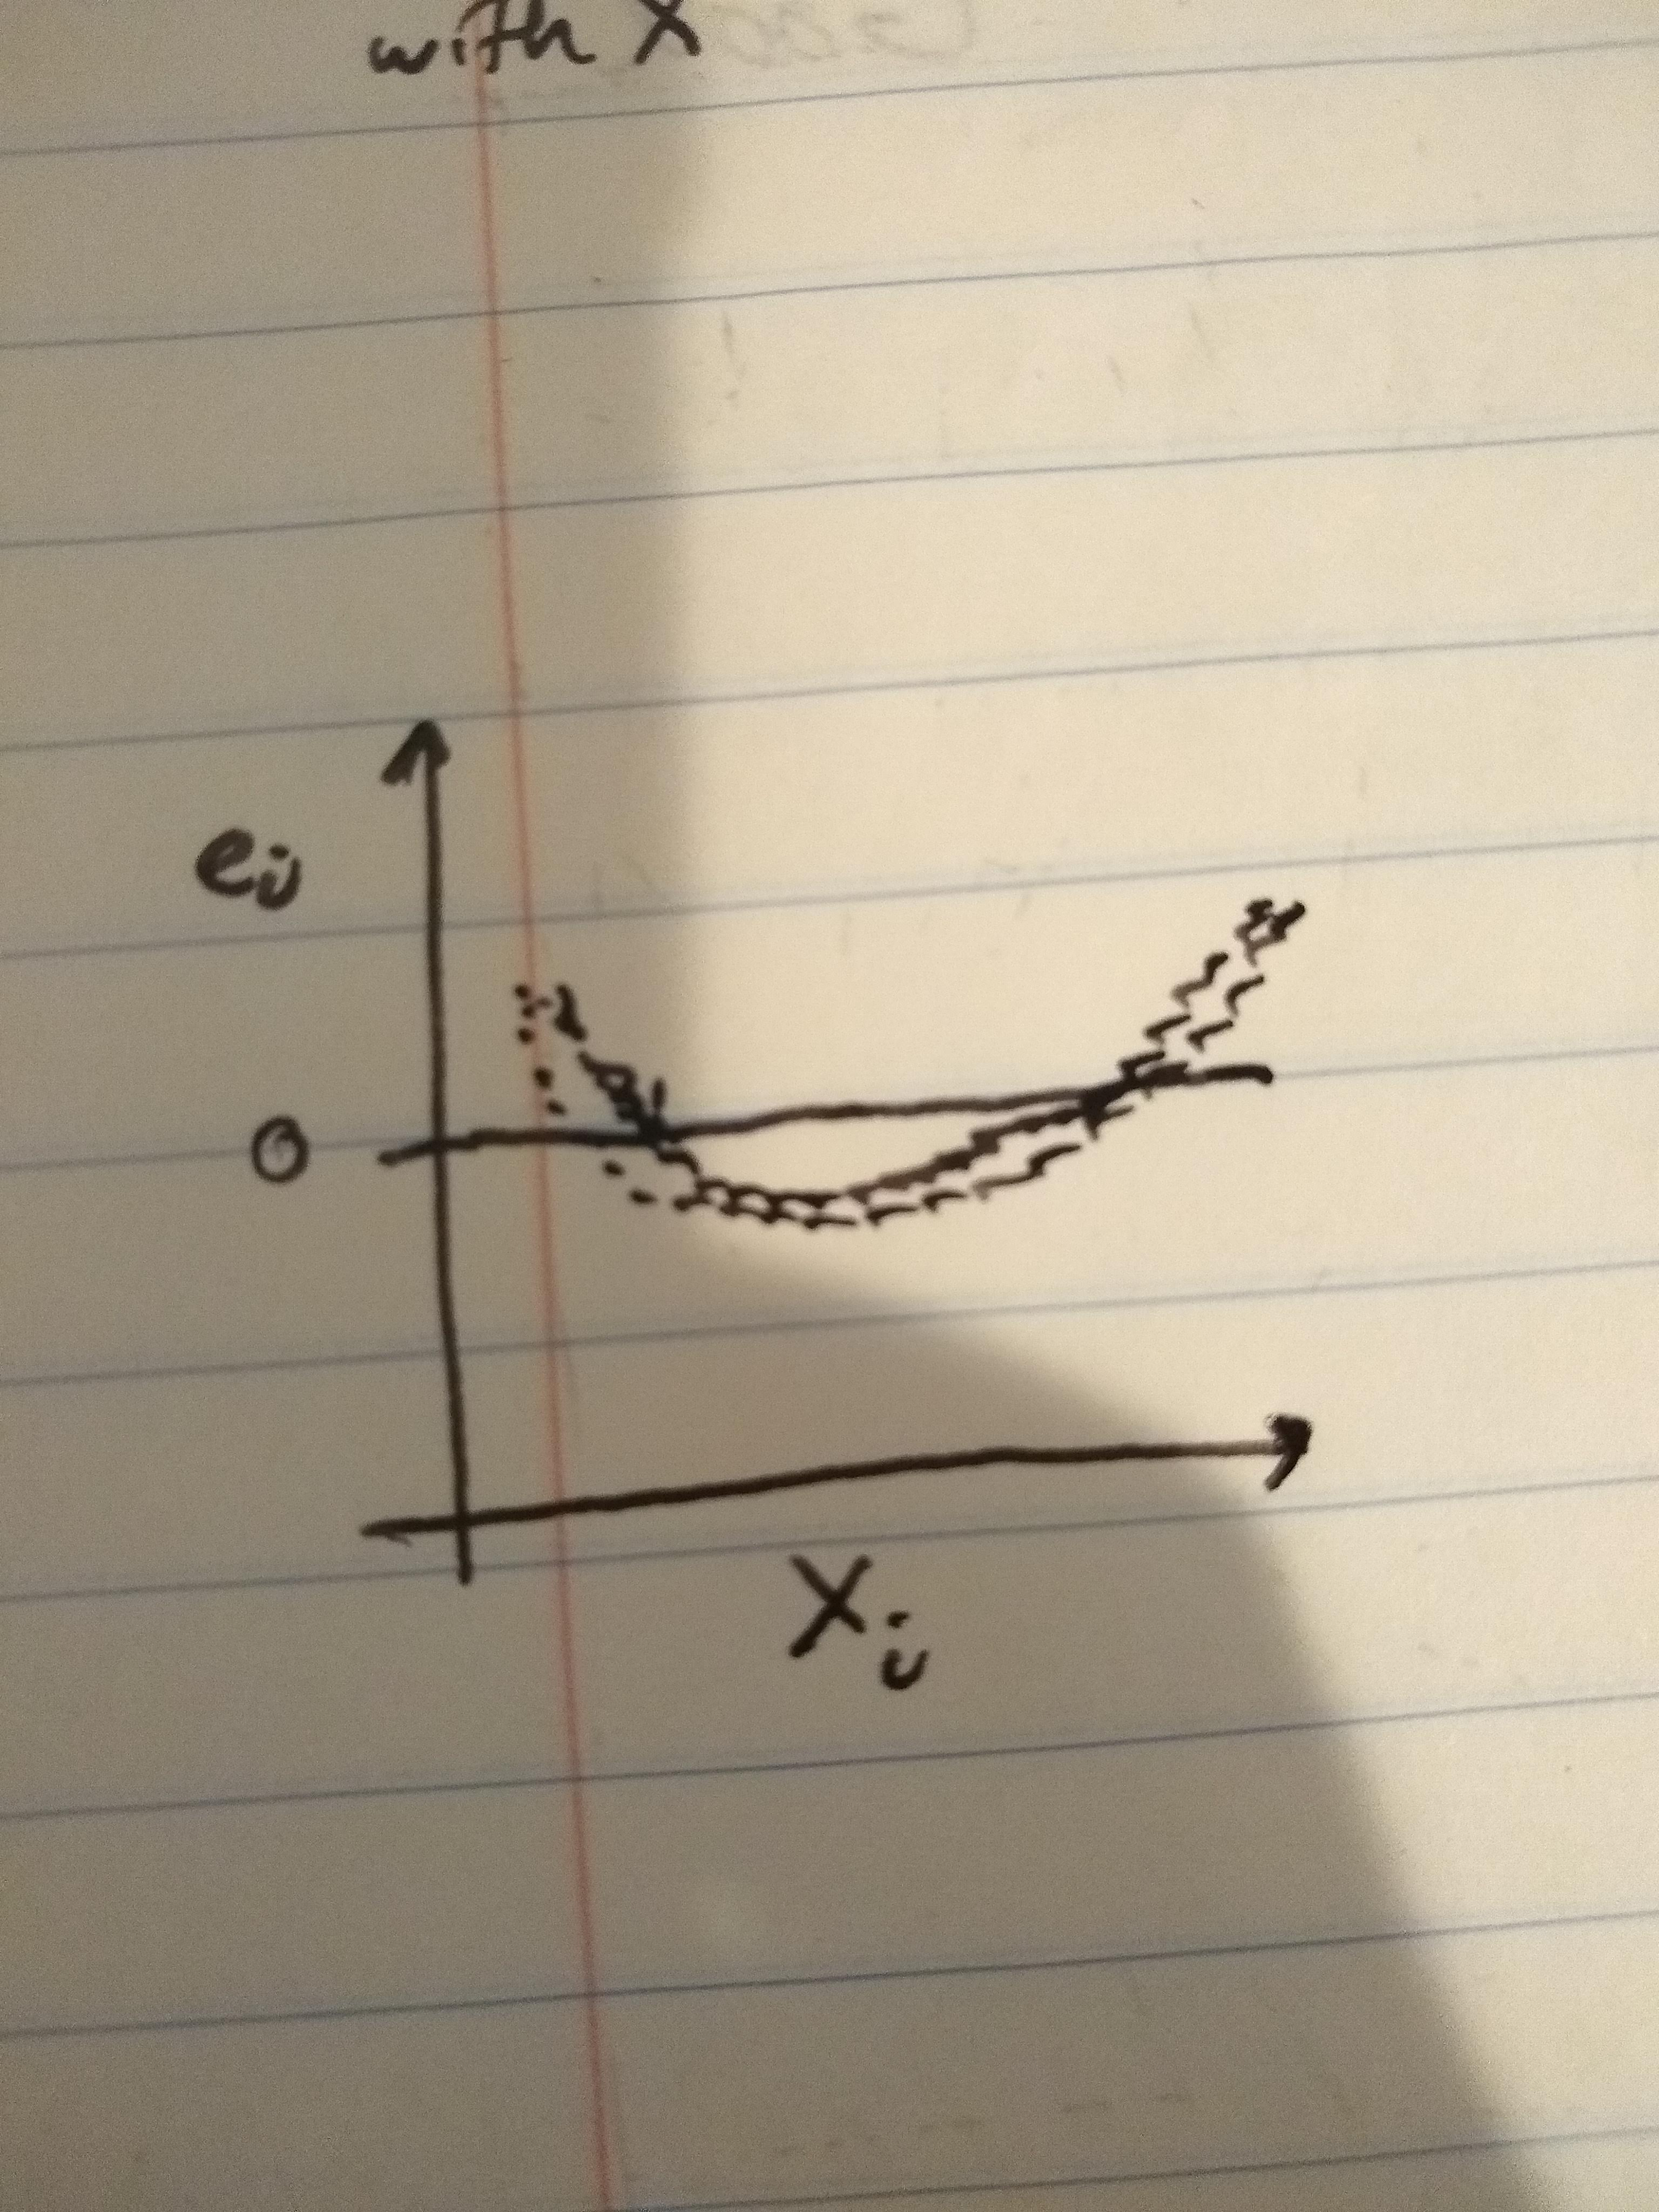
\includegraphics[width=.9\linewidth]{./images/3.2_2.jpg}
\caption{\label{fig:org0772d0d}
True Regression is Parabolic}
\end{figure}

\section{3.6}
\label{sec:org94baad3}
\subsection{a}
\label{sec:org225ce07}
\begin{quote}
Obtain the residuals and prepare a boxplot. What information is provided?
\end{quote}

The boxplot shows the median, quartiles, and min/max of the residual values from
the SLR Model: \(\hat{Y_{H}} = 168.6 + 2.0344 \times \text{Hours}\). This shows
that over 50\% of Residuals lie between -3 and 3 with the 50th percentile laying
near 0.


\begin{figure}[htbp]
\centering
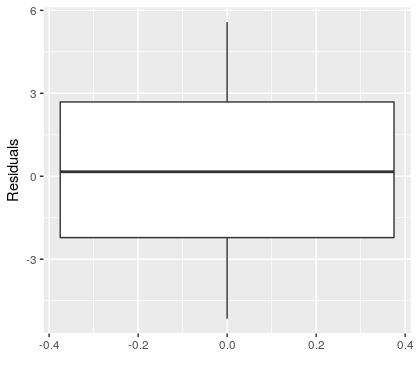
\includegraphics[width=.9\linewidth]{./images/3.6a.png}
\caption{Residual Boxplot}
\end{figure}

\subsection{b}
\label{sec:org4b8d097}
\begin{quote}
Plot the residuals against the fitted values to ascertain whether any departures
from the regression model are evident. State your findings
\end{quote}

There is a noticable wave-like pattern with the residuals that starts below \(Y =
0\) and \(X = 201.15\), rises above \(Y = 0\) at \(X = 217.425\), and dips below again
at the X values afterwards. This indicates that the regression function is \textbf{not}
linear, and that the error terms may not be independent.

\begin{figure}[htbp]
\centering
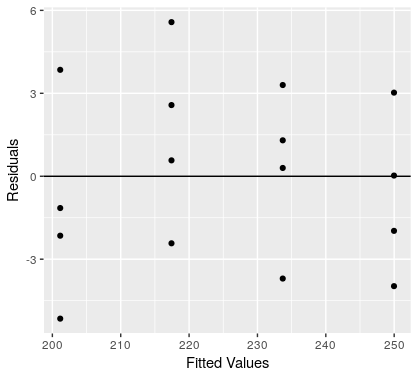
\includegraphics[width=.9\linewidth]{./images/3.6b.png}
\caption{\label{fig:org7998d56}
Residuals vs Fitted Values}
\end{figure}

\subsection{c}
\label{sec:org9dccc42}
\begin{quote}
Prepare a normal probability plot of the residuals. Also obtain the coefficient
of correlation between the ordered residuals and their expected values under
normality. Does the normality assumption appear to be reasonable here?
\end{quote}

There is not enough evidence to suggest that the residuals are not normal
(Shapiro-Wilk. p-value = 0.8914). The Normal Probability plot supports this
conclusion as well. Thus the normality assumption appears to be reasonable.

\begin{verbatim}
shapiro.test(x = plastic.model1$residuals)
#	Shapiro-Wilk normality test

#data:  plastic.model1$residuals
#W = 0.97348, p-value = 0.8914
\end{verbatim}

\begin{figure}[htbp]
\centering
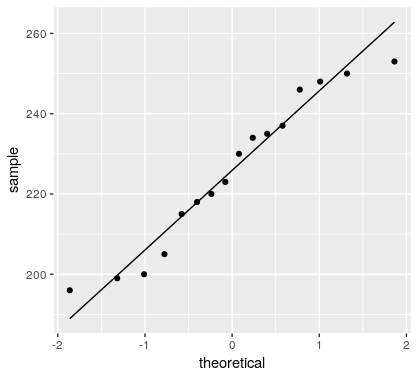
\includegraphics[width=.9\linewidth]{./images/3.6c.png}
\caption{\label{fig:org12ef483}
Normal Probability Plot}
\end{figure}

\subsection{e}
\label{sec:orga3e89e3}
\begin{quote}
Use the Brown-Forsythe test to determine whether or not the error variance
varies with the level of X. Divide the data into 2 groups, X <= 24 and X> 24.
State the decision rule and conclusion. Does your conclusion support your
preliminary findings in b?
\end{quote}

There is not enough evidence to suggest that data does not have constant
variance (Brown-Forsyth Levene's Test. p-value = 0.04065). Examining the
residual plot in B showed that variance was more or less constant so this
confirms the initial conclusion.

\begin{verbatim}
plastic$Group <- plastic$Hours <= 24
levene.test(y = plastic.model1$residuals, group = plastic$Group)

#	Modified robust Brown-Forsythe Levene-type test based on the absolute deviations from the median

#data:  plastic.model1$residuals
#Test Statistic = 0.73237, p-value = 0.4065
\end{verbatim}
\end{document}
